
\begin{enumerate}

\item A walking tour of K\"{o}nigsberg such as is described in this section,
or more generally, a circuit through an arbitrary graph that crosses each
edge precisely once and begins and ends at the same node is known as
an \index{Eulerian circuit} \emph{Eulerian circuit}.  An \index{Eulerian
path} \emph{Eulerian path} also crosses every edge of a graph exactly
once but it begins and ends at distinct nodes.  For each of the following
graphs determine whether an Eulerian circuit or path is possible, and if so,
draw it.

\begin{center}
\begin{picture}(0,0)%
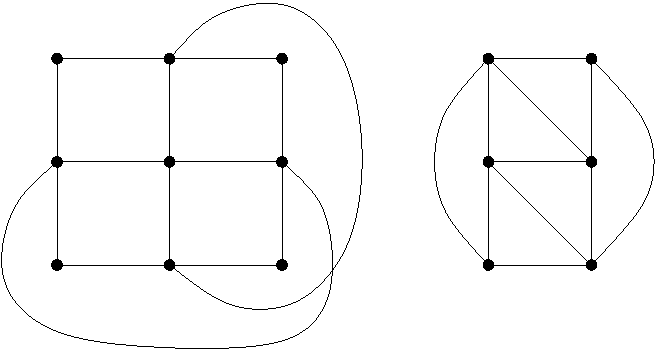
\includegraphics{./Euler_circuit_problems_a.pdf}%
\end{picture}%
\setlength{\unitlength}{3947sp}%
%
\begingroup\makeatletter\ifx\SetFigFont\undefined%
\gdef\SetFigFont#1#2#3#4#5{%
  \reset@font\fontsize{#1}{#2pt}%
  \fontfamily{#3}\fontseries{#4}\fontshape{#5}%
  \selectfont}%
\fi\endgroup%
\begin{picture}(5244,2786)(745,-2541)
\end{picture}%

\end{center}

\begin{center}
\begin{picture}(0,0)%
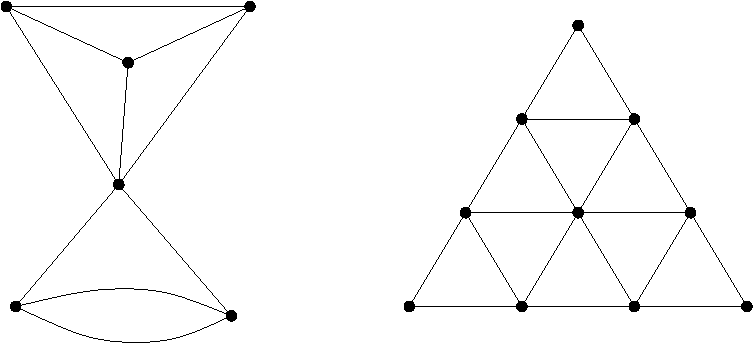
\includegraphics{./Euler_circuit_problems_b.pdf}%
\end{picture}%
\setlength{\unitlength}{3947sp}%
%
\begingroup\makeatletter\ifx\SetFigFont\undefined%
\gdef\SetFigFont#1#2#3#4#5{%
  \reset@font\fontsize{#1}{#2pt}%
  \fontfamily{#3}\fontseries{#4}\fontshape{#5}%
  \selectfont}%
\fi\endgroup%
\begin{picture}(6025,2749)(1226,-3136)
\end{picture}%

\end{center}

\item Complete the proof of the fact that ``Every graph has an even number
of odd nodes.''


\item Provide an argument as to why an $8 \times 8$ chessboard with 
two squares pruned from diagonally opposite corners cannot be tiled
with dominoes.

\item Prove that, if $n$ is odd, any $n \times n$ chessboard with 
a square the same color as one of its corners pruned can be tiled by
dominoes.

\item The five \index{tetromino} tetrominoes (familiar to players of the video game
Tetris) are relatives of dominoes made up of four small squares.

\begin{center}
\begin{picture}(0,0)%
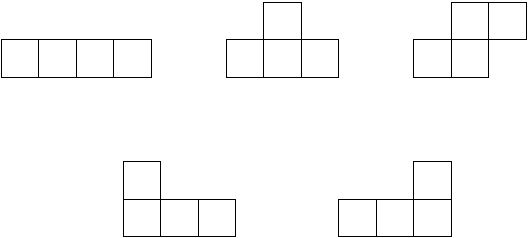
\includegraphics{figures/five_tetrominoes.pdf}%
\end{picture}%
\setlength{\unitlength}{3947sp}%
%
\begingroup\makeatletter\ifx\SetFigFont\undefined%
\gdef\SetFigFont#1#2#3#4#5{%
  \reset@font\fontsize{#1}{#2pt}%
  \fontfamily{#3}\fontseries{#4}\fontshape{#5}%
  \selectfont}%
\fi\endgroup%
\begin{picture}(4224,1899)(1189,-1948)
\end{picture}%

\end{center}

\noindent All together these five tetrominoes contain 20 squares
so it is conceivable that they could be used to tile a $4 \times 5$
chessboard.  Prove that this is actually impossible.

\item State necessary and sufficient conditions for the existence of
an Eulerian circuit in a graph.  

\item  State necessary and sufficient conditions for the existence of
an Eulerian path in a graph.  

\newpage

\item Construct magic squares of order 4 and 5.

\item A magic hexagon of order 2 would consist of filling-in
the numbers from 1 to 7 in the hexagonal array below.  The magic
condition means that each of the 9 ``lines'' of adjacent hexagons
would have the same sum.  Is this possible?

\begin{center}
\begin{picture}(0,0)%
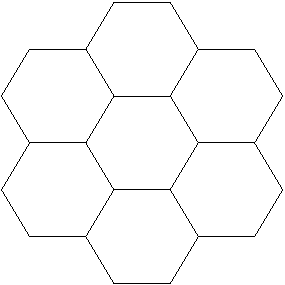
\includegraphics{figures/magic_hexagon.pdf}%
\end{picture}%
\setlength{\unitlength}{3947sp}%
%
\begingroup\makeatletter\ifx\SetFigFont\undefined%
\gdef\SetFigFont#1#2#3#4#5{%
  \reset@font\fontsize{#1}{#2pt}%
  \fontfamily{#3}\fontseries{#4}\fontshape{#5}%
  \selectfont}%
\fi\endgroup%
\begin{picture}(2274,2274)(2164,-3073)
\end{picture}%

\end{center}

\item Is there a magic hexagon of order 3?

\end{enumerate}



%% Emacs customization
%% 
%% Local Variables: ***
%% TeX-master: "GIAM-hw.tex" ***
%% comment-column:0 ***
%% comment-start: "%% "  ***
%% comment-end:"***" ***
%% End: ***

